\documentclass[20pt,landscape,footrule,headrule]{foils}
\usepackage[usenames]{color}
\usepackage[export]{adjustbox}
\usepackage{latexsym}
\usepackage{amsmath}
\usepackage{graphicx,color}  %needed to \includegraphics
\usepackage{amssymb}
\usepackage{multirow}
\usepackage{multicol}
\usepackage{polynom}
\newcommand{\newl}{\newline\newline}
\newcommand{\GN}{\mathbb{N}}
\newcommand{\GZ}{\mathbb{Z}}
\newcommand{\GQ}{\mathbb{Q}}
\newcommand{\GR}{\mathbb{R}}
\pagenumbering{arabic}

\newcommand{\crois}{\nearrow}
\newcommand{\decrois}{\searrow}

\newcommand{\cch}{\setlength{\unitlength}{0.2mm}
\begin{picture}(25,25)
\thicklines
\curve(0,0,15,7,25,23)
\end{picture}}

\newcommand{\ccb}{\setlength{\unitlength}{0.2mm}
\begin{picture}(25,25)
\thicklines
\curve(0,0,7,15,25,23)
\end{picture}}

\newcommand{\dch}{\setlength{\unitlength}{0.2mm}
\begin{picture}(25,25)
\thicklines
\curve(0,23,10,7,25,0)
\end{picture}}

\newcommand{\dcb}{\setlength{\unitlength}{0.2mm}
\begin{picture}(25,25)
\thicklines
\curve(0,23,15,18,25,0)
\end{picture}}

\usepackage{epic}
\usepackage{curves}


\usepackage[utf8]{inputenc}
\usepackage{xcolor}
\usepackage{newunicodechar}

\newcommand\Warning{%
 \makebox[1.4em][c]{%
 \makebox[0pt][c]{\raisebox{.1em}{!}}%
 \makebox[0pt][c]{\color{red}\Large$\bigtriangleup$}}}%


\newcommand{\localtextbulletone}{{\raisebox{.45ex}{\rule{.6ex}{.6ex}}}}
\renewcommand{\labelitemi}{\localtextbulletone}

\DeclareMathOperator{\pgdc}{pgdc}
\DeclareMathOperator{\card}{card}
\DeclareMathOperator{\sgn}{sgn}
\DeclareMathOperator{\SG}{SG}
\DeclareMathOperator{\lo}{lo}
\DeclareMathOperator{\IC}{I.C.}
\DeclareMathOperator{\ID}{I.D.}
\DeclareMathOperator{\IH}{I.H.}
\DeclareMathOperator{\IB}{I.B.}
\DeclareMathOperator{\INF}{INFL}
\DeclareMathOperator{\SC}{S.C.}
\DeclareMathOperator{\SP}{S.P.}
\DeclareMathOperator{\cosec}{cosec}
\DeclareMathOperator{\cotg}{cotg}
\DeclareMathOperator{\tg}{tg}
\DeclareMathOperator{\tgh}{tgh}
\DeclareMathOperator{\sech}{sech}
\DeclareMathOperator{\cosech}{cosech}
\DeclareMathOperator{\cotgh}{cotgh}

%%%%%%%%%%%%%%%%%%%%%%%%%%%%%%%%%%%%%%%%%%%%%

%%%%%%%%%%%%%%%%%%%%%%%%%%%%%%%%%%%%%%%%%%%%%%%%%%%%%%%

\input def

%\usepackage[T1]{fontenc}

\def\filedate{Fall 2020}
\def\fh{\foilhead}
\def\me{P.Boily (uOttawa) \\ with O.Leduc, A.Macfie, A.Maheshwari, M.Pelletier}
\def\code{MAT 4376/5314E \\ Techniques of Data Analysis}
\def\codee{MAT 4376/5314E}
\def\descr{Techniques of Data Analysis}
\def\lec{}
\def\sec{4}
\def\sections{}
\def\sectitle{Feature Selection and Dimension Reduction}
\def\unitofstudy{\codee\ -- \descr}
\def\mc{\mathcal}
\def\rfh{\rotatefoilhead}
\title{\code \\ \ \\  Module \sec\\ \sectitle}
\author{\me}
\date{\filedate}
\definecolor{burgundy}{rgb}{0.6, 0.0, 0}
\definecolor{bleudefrance}{rgb}{0, 0, 0.6}
\definecolor{darkestgreen}{rgb}{0, 0.6, 0}
\definecolor{grey}{rgb}{0.5, 0.5, 0.5}
%\setlength{\parskip}{50pt}

\begin{document}
\maketitle \MyLogo{Feature Selection and Dimension Reduction}
\leftheader{\unitofstudy} \rightheader{Module \sec\ -- \sectitle}
\rightfooter{\quad\textsf{\thepage}} % this is the default

\fh{\textcolor{grey}{Outline}}
\noindent Data mining is the collection of processes by which we extract actionable  insights from data. Inherent in this definition is the idea of \textbf{data reduction}: useful insights (whether in the form of summaries, sentiment analyses, etc.) ought to be ``smaller'' and ``more organized'' than the original raw data. The challenges presented by high data dimensionality must be addressed in order to achieve insightful and interpretable analytical results. \newl Scenario -- NHL Game and Data Reduction (p.\pageref{sc1})
\newl 4.1 -- Dimension Reduction (p.\pageref{4.1}) \\
\small\textcolor{white}{ab} \localtextbulletone\ The Curse of Dimensionality (p.\@\pageref{4.1.1}) \\ \textcolor{white}{ab} \localtextbulletone\ Principal Component Analysis (p.\@\pageref{4.1.2}) \\ \textcolor{white}{ab} \localtextbulletone\ The Manifold Hypothesis  (p.\@\pageref{4.1.3}) \normalsize\newpage\ \\ \noindent
4.2 -- Feature Selection (p.\pageref{4.2})\\
\small\textcolor{white}{ab} \localtextbulletone\ Filter Methods (p.\@\pageref{4.2.1}) \\ \textcolor{white}{ab} \localtextbulletone\ Wrapper Methods (p.\@\pageref{4.2.2}) \\ \textcolor{white}{ab} \localtextbulletone\ Subset Selection Methods (p.\@\pageref{4.2.3}) \\ 
\textcolor{white}{ab} \localtextbulletone\ Regularization Methods (p.\@\pageref{4.2.4}) \\ \textcolor{white}{ab} \localtextbulletone\ Supervised and Unsupervised Methods (p.\@\pageref{4.2.5})\normalsize\newl  
4.3 -- Advanced Topics (p.\pageref{4.3}) \\ 
\small\textcolor{white}{ab} \localtextbulletone\ Singular Value Decomposition (p.\@\pageref{4.3.1}) \\ \textcolor{white}{ab} \localtextbulletone\ Spectral Feature Selection (p.\@\pageref{4.3.2}) \\ \textcolor{white}{ab} \localtextbulletone\ Uniform Manifold Approximation and Projection  (p.\@\pageref{4.3.3}) \normalsize
\fh{\textcolor{grey}{Scenario -- NHL Game and Data Reduction}} \label{sc1}
\newpage
\begin{center}
    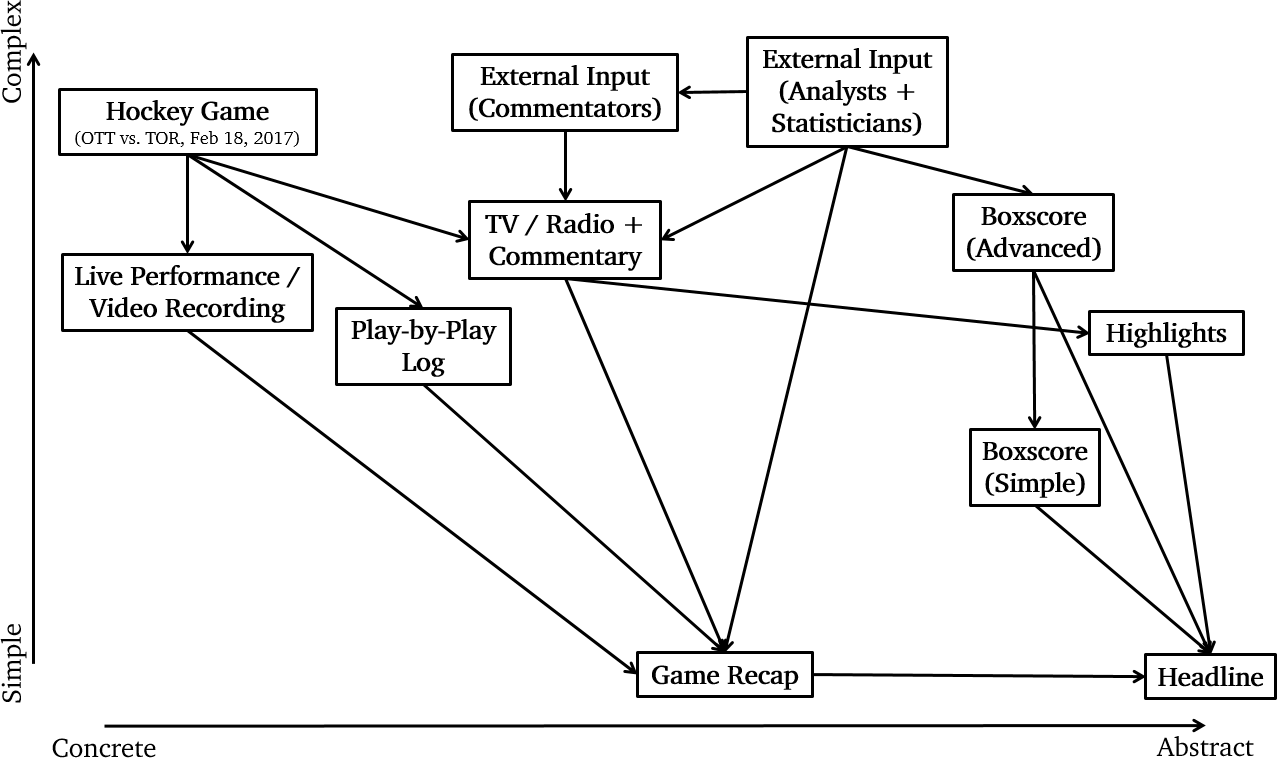
\includegraphics[width=0.95\textwidth]{Images/TM_Brain_Hockey.png} \\  Schematic diagram of data reduction -- professional hockey game.\normalsize
\end{center}
\newpage\ \\
\begin{center}
        \includegraphics[width=0.65\textwidth]{Images/Game_Summary_Numbers.png} \\  Boxscore, Ottawa Senators @ Toronto Maple Leafs, 18-02-2017 (espn.com) \normalsize
        \newl\newline \Large
        \textbf{Sens rally after blowing lead, \\ beat Leafs, gain on Habs.} \normalsize \\ Headline, Associated Press, 18-02-2017
\end{center}
\newpage 
\begin{center}
\includegraphics[width=0.57\textwidth]{Images/20162017-20861-all} \\  \includegraphics[width=0.57\textwidth]{Images/20162017-20861-cfdiff-all} \\ Unblocked shot heatmap and Corsi gameflow chart (Natural Stat Trick).
\end{center}
\newpage
\begin{center}
    \includegraphics[width=\textwidth]{Images/data_reduction.png} \\  Schematic diagram of data reduction -- general problem (Schellinck).\normalsize
\end{center}

\fh{\textcolor{grey}{4.1 -- Dimension Reduction}} \label{4.1}

\fh{4.1.1 -- The Curse of Dimensionality} \label{4.1.1}

\newpage \ \\ 
\begin{center}
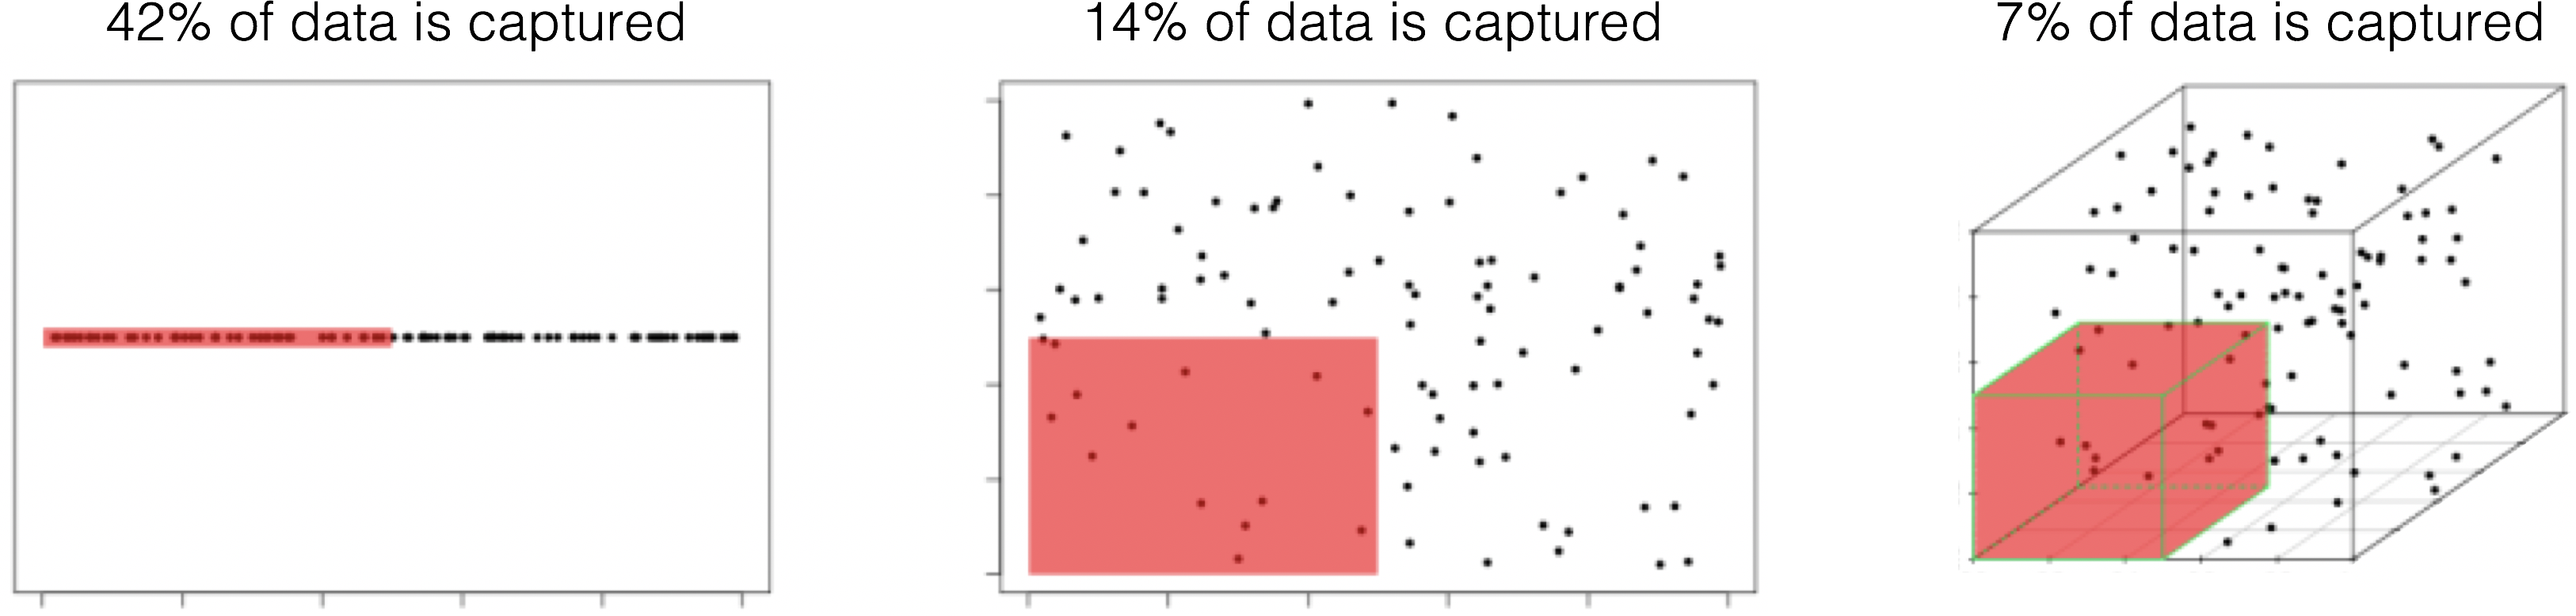
\includegraphics[width=\textwidth]{Images/COD.png}\end{center} Illustration of the CoD; $N=100$ observations are uniformly distributed on the unit hypercube $[0,1]^d$, $d=1, 2, 3$. \newl The red regions represent the smaller hypercubes $[0,0.5]^d$, $d=1,2,3$. \newl The percentage of captured datapoints is seen to decrease with an increase in $d$ (from simplystatistics.com). \normalsize
\fh{4.1.2 -- Principal Component Analysis} \label{4.1.2}
\newpage\ \\ 
\begin{center}
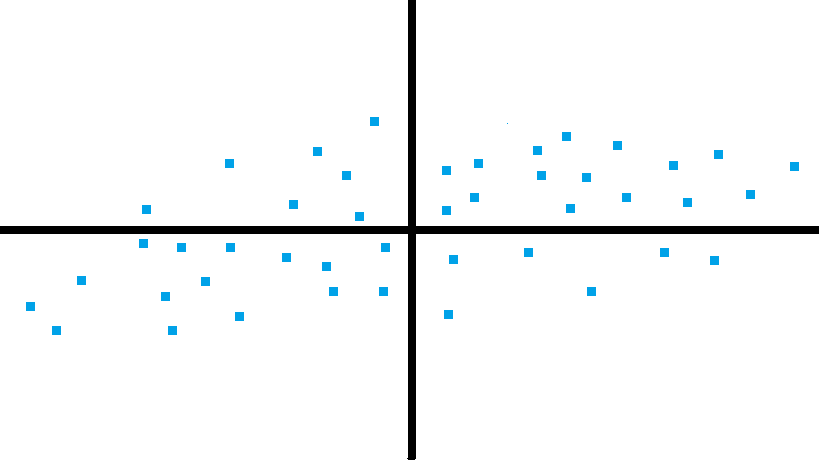
\includegraphics[width=0.3\textwidth]{Images/PC1.png}\quad
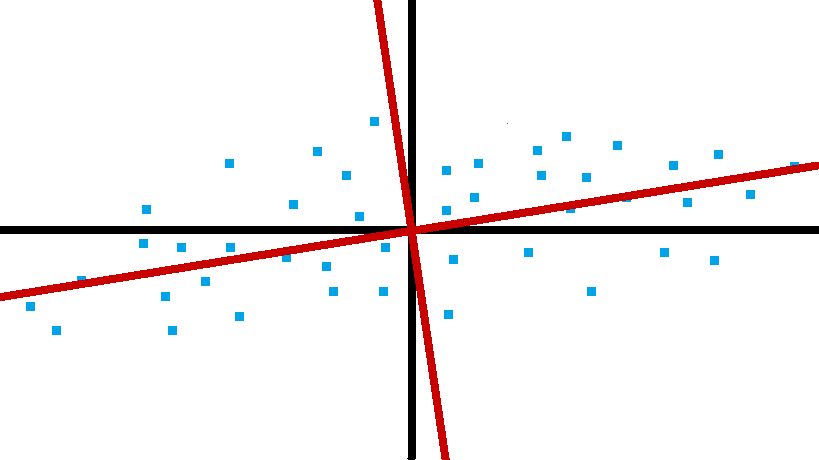
\includegraphics[width=0.3\textwidth]{Images/PC2.png}\\
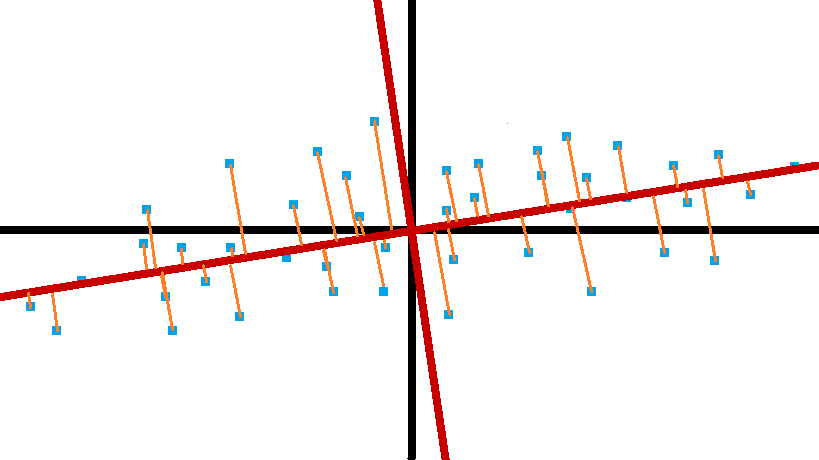
\includegraphics[width=0.3\textwidth]{Images/PC3.png}\quad
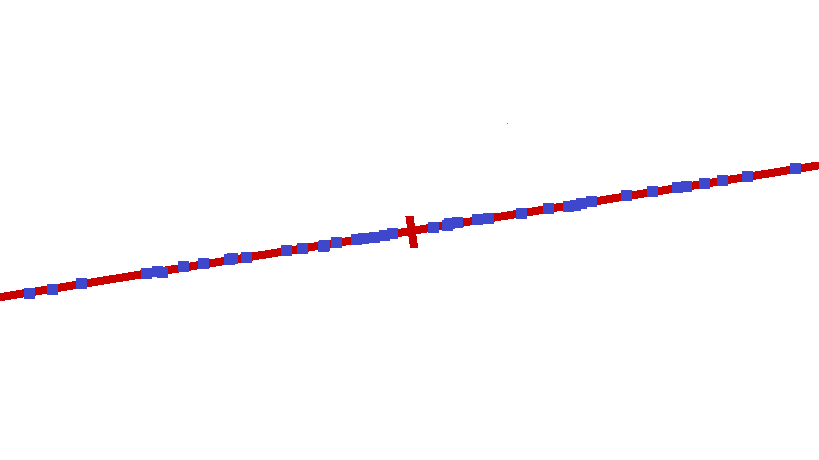
\includegraphics[width=0.3\textwidth]{Images/PC4.png}
\end{center} Illustration of PCA on an artificial 2D dataset. The red axes  represent the axes of the best elliptic fit. Removing the minor axis by projecting the points on the major axis leads to a dimension reduction and a (small) loss of information. \newpage\ \\ \begin{center}
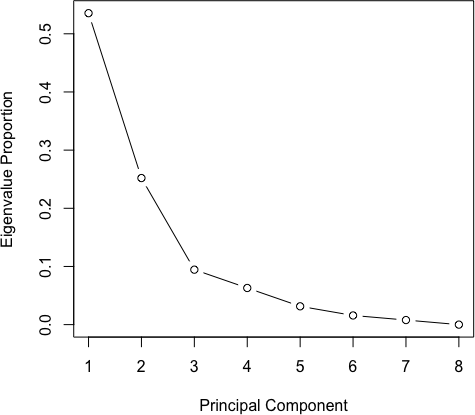
\includegraphics[width=0.24\textwidth]{Images/Eigenvalue_plot1.png}\ 
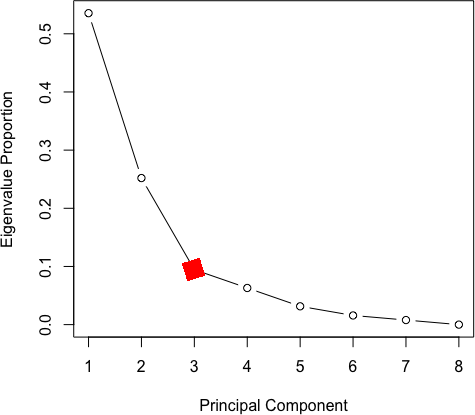
\includegraphics[width=0.24\textwidth]{Images/Eigenvalue_plot2.png}\ 
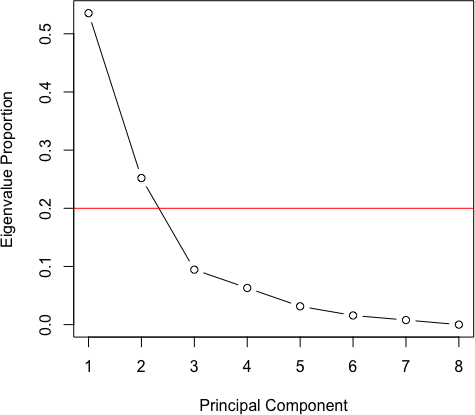
\includegraphics[width=0.24\textwidth]{Images/Eigenvalue_plot3.png}\ 
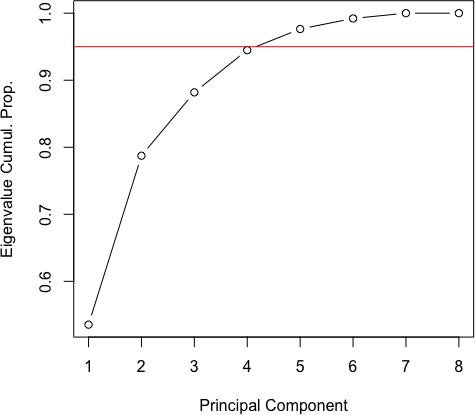
\includegraphics[width=0.24\textwidth]{Images/Eigenvalue_plot4.png}
\end{center}
The proportion of the variance explained by each (ordered) component is shown in the first $3$ charts; the cumulative proportion is shown in the last chart. \newl The kink method is shown in the second image, the individual threshold component in the third, and the cumulative proportion in the fourth.

\fh{4.1.3 -- The Manifold Hypothesis} \label{4.1.3}
\newpage\ \\ 
\begin{center}
  \includegraphics[width=\textwidth]{FSDR/Images/Spiral.png}\end{center}
  Unfolding of a high-dimensional manifold (Tenenbaum, Silva, Langford).
  
  \newpage
  \begin{center}
    \adjincludegraphics[trim={0 {0.5\height} 0 0}, clip, width=0.6\textwidth]{FSDR/Images/FacesNumbers.png}
    \end{center}
  Plots showing degrees of freedom manifolds for images of faces -- 3D object (Tenenbaum, Silva, Langford).    \newpage
    \begin{center}
    \adjincludegraphics[trim={0 0 0 {0.5\height}}, clip, width=0.6\textwidth]{FSDR/Images/FacesNumbers.png}
    \end{center}
   Plots showing degrees of freedom manifolds for images of handwritten digits (Tenenbaum, Silva, Langford).
   \newpage 
\begin{center}
  \includegraphics[width=0.75\textwidth]{FSDR/Images/S-Shape.png}
\end{center}
Comparison of manifold learning methods on an artificial dataset (Cayton).
\newpage \ \\ 
\begin{center}
 \includegraphics[width=0.77\textwidth]{FSDR/Examples/MNISTData.png}
\end{center}
Sample from the MNIST dataset (LeCun, Cortes, Burges).
\newpage
\begin{center}
  \includegraphics[width=7.8cm]{FSDR/Examples/LLEMNIST.png} \includegraphics[width=7.8cm]{FSDR/Examples/HLLEMNIST.png} \includegraphics[width=7.8cm]{FSDR/Examples/ISOMAPMNIST.png}  \includegraphics[width=7.8cm]{FSDR/Examples/tSNEMNIST0-5.png}
\end{center}
 Manifold learning on digits $0-5$: LLE, Hessian LLE, Isomap, $t-$SNE. 
\fh{\textcolor{grey}{4.2 -- Feature Selection}} \label{4.2}

\fh{4.2.1 -- Filter Methods} \label{4.2.1}
\newpage
\begin{center}
  \includegraphics[width=0.95\textwidth]{FSDR/Images/salary1.png} \\ \includegraphics[width=0.95\textwidth]{FSDR/Images/salary2.png} \\ 
Summary statistics for the salary dataset; two-way tables use decile data.\end{center}
\newpage\ \begin{center}  \includegraphics[width=6cm]{FSDR/Images/Hair_bar.png} \quad \includegraphics[width=6cm]{FSDR/Images/Age_hist.png} \\ \includegraphics[width=6cm]{FSDR/Images/Height_hist.png} \quad   \includegraphics[width=6cm]{FSDR/Images/Salary_hist.png}\\
Univariate distributions (hair colour, age, height, salary). \end{center}
\newpage\  
\begin{center}
  \includegraphics[width=0.45\textwidth]{FSDR/Images/MITable.png}
  \end{center}
Mutual information obtained about each predictor after observing the target response $Y$ (salary). \newl The percentage decrease in entropy after having observed $Y$ is shown in the column ``Ratio.'' \newl Raw IG numbers would seem to suggest that Gender has a small link to Salary; the Ratio numbers suggest that this could be due to the way the Age and Height levels have been categorized (deciles).
\fh{4.2.2 -- Wrapper Methods} \label{4.2.2}

\newpage 
\begin{center}
  \includegraphics[width=0.8\textwidth]{FSDR/Images/wrapperprocess.png}
  \end{center} 
Feature selection process for classification wrapper methods (Aggarwal). 


\fh{4.2.3 -- Subset Selection Methods} \label{4.2.3}

\fh{4.2.4 -- Regularization Methods} \label{4.2.4}

\fh{4.2.5 -- Supervised and Unsupervised Methods} \label{4.2.5}


\fh{\textcolor{grey}{4.3 -- Advanced Topics}} \label{4.3}

\fh{4.3.1 -- Singular Value Decomposition} \label{4.3.1}

\newpage\ \\
\begin{center}
\includegraphics[width=0.9\textwidth]{Images/svd1.png} \\ (modified from Leskovec, Rajaraman, Ullman) \end{center}
\newpage \ \\ 
\begin{center}
 \includegraphics[width=0.32\linewidth]{Images/maingray.png} \hfill
   \includegraphics[width=0.32\linewidth]{Images/main10.png}  \hfill \includegraphics[width=0.32\linewidth]{Images/main50.png} 
\end{center}
Image reconstruction: $d=1400$ (left), $d=10$ (middle), $d=50$ (right); Llewellyn and Gwynneth Rayfield.
\newpage \ \\ 
\begin{center}
\includegraphics[width=0.8\linewidth]{Images/wpwpt1.png}
\end{center}

\newpage\ 
\begin{center}
\includegraphics[width=0.5\textwidth]{Images/wpwpt4.png}
\end{center}
\newpage\ 
\begin{center}\includegraphics[width=0.4\textwidth]{Images/wpwpt3.png}
\end{center}
\newpage\ 
\begin{center}
\includegraphics[width=\linewidth]{Images/wpwpt2.png}
\end{center}



\fh{4.3.2 -- Spectral Feature Selection} \label{4.3.2}
\newpage \ 
    \begin{center}\includegraphics[width=0.7\textwidth]{Images/plot_exemple1.png}\\
Scatter plot of the example data $\mathbf{X}$.
\end{center}
\newpage 
\begin{center}
    \includegraphics[width=0.7\linewidth]{Images/graph_exemple.png}
    \end{center}
Graph representation of $\mathbf{X}$, using a RBF similarity matrix with $\sigma=0.5$. The graph has $6$ nodes, one for each observation. The edges with weights below a certain threshold ($\tau=0.01$) are not displayed.

\newpage\ 
\begin{center}
    \includegraphics[width=0.7\textwidth]{Images/example1.png}\\
    Scatter plot of data with $3$ different generative mechanism.
    \end{center}
    
\newpage
\begin{center}    \includegraphics[width=0.7\textwidth]{Images/spectrum_L.png} \\
Contour plot of the eigenvectors corresponding to $6$ eigenvalues.
\end{center}
\newpage
\begin{center}
    \includegraphics[width=0.7\textwidth]{Images/eig_comp_plot.png}
\\    Value of each eigenvector component (one for each observation) associated to $\lambda_1$, $\lambda_2$, $\lambda_3$, and $\lambda_{20}$.
\end{center}

\newpage\ 
\begin{center}
    \includegraphics[width=0.7\textwidth]{Images/useless_ex.png}
\\ Value of $\mathbf{f}_i$ component (one for each observation), for $i=1, 2, 3$.
\end{center}

\newpage\  
\begin{center}
    \includegraphics[width=0.65\textwidth]{Images/noise_L.png} \\
Effect of noise on the eigenvalues of the normalized Laplacian.
\end{center}

\newpage
\begin{center}
    \includegraphics[width=0.65\textwidth]{Images/gamma_effect.png} \\ 
Effect of different regularization functions on a the eigenvalues of the Laplacian of a noisy dataset.
\end{center}

\fh{4.3.3 -- Uniform Manifold Approximation and Projection} \label{4.3.3}

\newpage  \begin{center}\includegraphics[width=0.9\textwidth]{Images/reducers.png}  
\end{center}
\end{document}


